%%%%%%%%%%%%%%%%%%%%%%%%%%%%%%%%%%%%%%%%%%%%%%%%%%%%%%%%%%%%%%%%%
%
% Project     : Bachelorarbeit
% Title       : Machbarkeitsanalyse für eine ressourcenorientierte Schnittstelle zur Verarbeitung grundlegender Probleme der Informatik
% File        : architektur.tex Rev. 01
% Date        : 01.03.2015
% Author      : Raffael Santschi
%
%%%%%%%%%%%%%%%%%%%%%%%%%%%%%%%%%%%%%%%%%%%%%%%%%%%%%%%%%%%%%%%%%

\chapter{Konzept der Schnittstelle \resultAssignment{[R4]}}\label{chap.architektur}
In diesem Kapitel wird auf die Strukur und das Konzept der Schnittstelle eingegangen. Dieses Konzept legt die Grundlage für die Umsetzung und entscheidet somit, ob die 
Aufgabe gelöst werden kann.

\section{Übersicht}\label{architektur_uebersicht}
Die Systemumgebung (siehe Abbildung \ref{fig:system_scope}) hat zwei Berührungspunkte zur Aussenwelt. Der eine ist zum Nutzer hin, der andere zu einem Verarbeitungssystem. 
Um die Daten zu speichern, wird eine Datenbank benötigt. Das ermöglicht einen asynchronen Ablauf und ein mehrfaches Abfragen der Daten.
\begin{figure}[h]
\centering
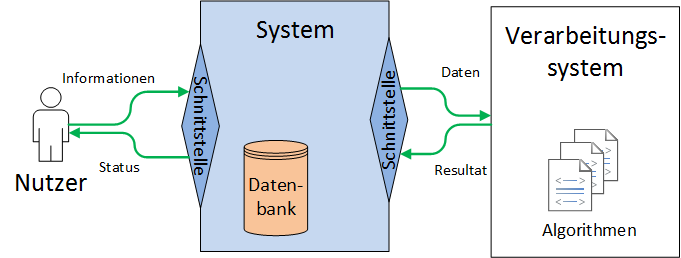
\includegraphics[scale=0.8]{images/visio/Systemscope.png}
\caption[System Übersicht]{System Übersicht \selfmade{}}
\label{fig:system_scope}
\end{figure}

\section{Konzept}\label{arch_backend}
Das Konzept sollte simpel und flexibel sein, damit das System möglichst schnell erweitert werden kann. Beim Betrachten der Probleme und der Abläufe wurde bemerkt, dass die Vorgänge 
Ähnlichkeiten aufweisen. Die Daten werden angenommen und für einen bestimmten Algorithmus aufbereitet. Das Verarbeitungssystem schickt das Resultat zurück und dieses wird dann 
wieder umgewandelt, so dass es für den Nutzer brauchbar ist. Es finden zwei Umwandlungen statt. Die Umwandlungen an sich sind von Problem zu Problem verschieden, es gibt jedoch 
auch dort gewisse Ähnlichkeiten. In \autoref{fig:architektur} wird der Aufbau des Systems gezeigt. Die  \gls{domainlanguage} des Nutzers wird mit Hilfe der Controller, Entities und 
den Translators auf die \gls{domainlanguage} der Algorithmen abgebildet.

\begin{figure}[h]
\centering
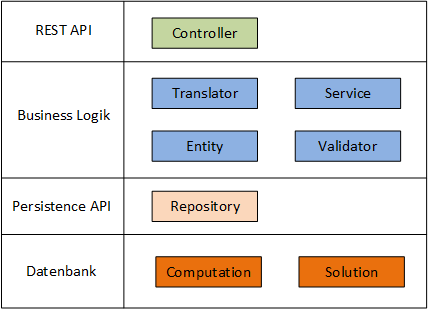
\includegraphics[scale=0.8]{images/visio/architektur_db.png}
\caption[Architekturaufbau des Systems]{Architekturaufbau des Systems \selfmade{}}
\label{fig:architektur}
\end{figure}
 
\FloatBarrier
\subsection{REST API}
Für die Schnittstelle wird ein \gls{rest} \gls{api} erstellt, welches die nötigen Funktionen bietet. Das \gls{api} funktioniert nach dem De-facto-Standard 
(siehe \cite{wiki_restful}). Falls Fehler auftreten, werden die \gls{http_statuscode} verwendet, um diese an den Aufrufer weiterzugeben.

\subsection{Business Logik}
Die Business Logik besteht aus Translator, Service, Entity und Validator von den jeweiligen Problemen. 
\paragraph{Translator}
Es gibt jeweils ein `ComputationTranslator' für die Umwandlung vom Nutzer hin zum Algorithmus und einen `SolutionTranslator' für die Umwandlung vom Algorithmus zurück in das System. In den 
Translators steckt die ganze Logik. Hier fliesst ein, wie der Algorithmus die Daten für die Verarbeitung benötigt und wie das Resultat zurück kommt. Es wäre zum Beispiel möglich, die Daten in 
Kombinationen für einen evolutionären Algorithmus umzuwandeln, so würde allenfalls ein generischer Algorithmus für alle Probleme ausreichen. Ebenfalls möglich wäre eine Umwandlung des 
Stundenplanproblems auf ein Knotenfärbungsproblem und somit könnte der gleiche Algorithmus angesprochen werden (vergleiche \cite{timetabling_abdullah}). Die Möglichkeiten mit dem 
Konzept der Translators ist sehr vielfälltig. Zusätzlich kann im Translator das Resultat mit zusätzlichen Informationen, zum Beispiel Statistiken, angereichert werden.
\paragraph{Service}
Der Service kann sehr generisch gehalten werden und benötigt keine problemspezifisches Methoden. 
\paragraph{Entity}
Die Entitäten sind von Problem zu Problem unterschiedlich. Es muss analysiert werden, wie die Parameter am besten eingegeben werden und wie diese dann vom Algorithmus 
gebraucht werden. 
\paragraph{Validator}
Der Validator entscheidet, ob eine Lösung gültig ist oder nicht. Wie bereits im \autoref{cat_theo_inf} erklärt, kann jedes NP-vollständige Problem in \glslink{polynomialzeit}{polynomialer} Zeit validiert werden.

\subsection{Persistance API}
Die Abstraktion der Datenbank wird mittels eines Persistance APIs, welches mit der Datenbank interagiert, realisiert. Dieses API ist für das Laden und Speichern der Daten 
verantwortlich und bietet die Möglichkeit, spezifische Abfragen auszuführen.

\subsection{Datenbank}
Jedes Problem hat seine eigene Ausprägung von Computation und Solution, welche abgespeichert werden müssen. Die Datenbank sollte, wenn möglich, eine ähnliche Flexibilität, wie 
das Programm selber, aufweisen. Die Vorgänge benötigen keine Transaktionen und sind zum grossen Teil nur Einfüge-Operationen, nur selten wird ein Eintrag geändert. Die Daten werden 
immer in der Nutzer-Sicht gespeichert.

\newpage
\subsection{Ablauf}
In \autoref{fig:workflow} wird der Ablauf des ganzen Vorganges und die Interaktion mit dem Nutzer und dem Verarbeitungssystem verdeutlicht. Die Translators, welche in dem 
Prototyp verwendet werden, sind nur eine Möglichkeit, welche dieses Konzept bietet. Generell baut dieses Konzept auf eine pre- und post-Aktion vor bzw. nach dem Starten des Algorithmus 
auf.

\begin{figure}[h]
\centering
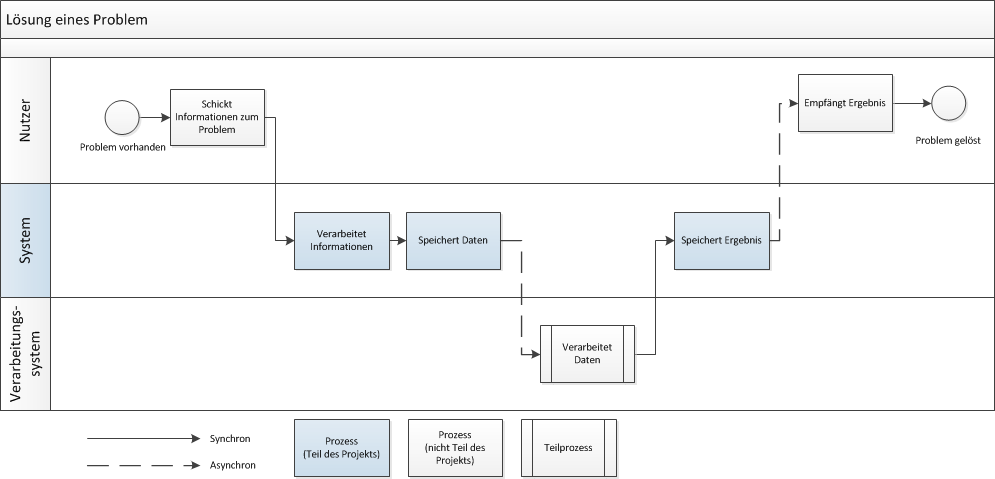
\includegraphics[scale=0.605]{images/visio/workflow.png}
\caption[Flussdiagramm des Arbeitsablaufs]{Flussdiagramm des Arbeitsablaufs \selfmade{}}
\label{fig:workflow}
\end{figure}

\FloatBarrier
\newpage

Die \autoref{fig:sequenz_diagramm_start} zeigt das Sequenzdiagramm für den Start eines beliebigen Problems, alle Komponenten mit '\{Problem\}' sind spezifische Problem-Komponenten, 
die anderen sind generische. Bei Speichern einer Berechnung wird der Status 'CREATED' gesetzt. Nach dem Speichern wird über die `Solver'-Komponente asynchron das Verarbeitungssystem 
gestartet und der Status auf 'STARTED' gesetzt. Das Verarbeitungssystem holt sich die benötigten Informationen. Der Controller lädt das Problem vom Service, dieser wiederum lädt es vom 
Repository und wandelt es für den Algorithmus um.

\begin{figure}[h]
\centering
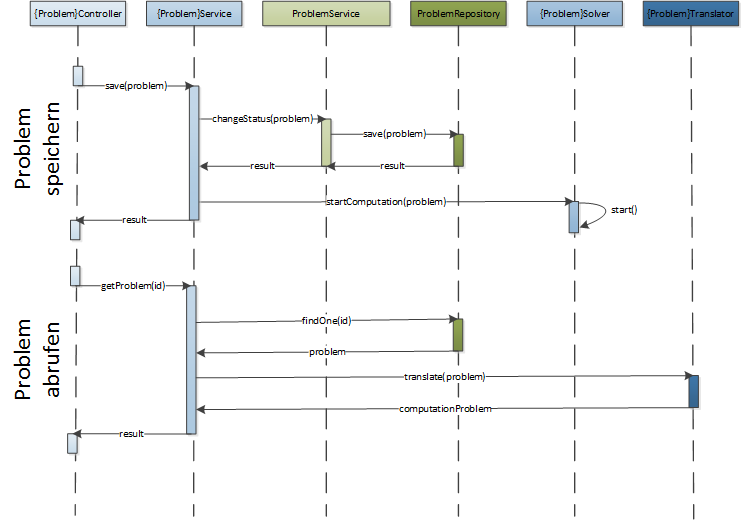
\includegraphics[scale=0.74]{images/visio/sequenz_diagramm_start.png}
\caption[Start eines beliebigen Problemes]{Start eines beliebigen Problemes \selfmade{}}
\label{fig:sequenz_diagramm_start}
\end{figure}

\newpage

Die \autoref{fig:sequenz_diagramm_result} zeigt das Sequenzdiagramm für das Abspeichern eines Resultates einer beliebigen Berechnung. Bei einem Speicheraufruf wird zuerst das Problem 
geladen, danach wird die Lösung vom Algorithmus mit Hilfe der Eingabeparameter transferiert und vom Validator validiert. Nun wird anhand des Resultattypes der Status der Berechnung 
abgeändert. Das Resultat wird mit dem Ergebnis der Validierung in die Datenbank gespeichert. Wenn der Nutzer den Status einer Berechnung abruft, fragt der Controller über den 
Service den Status ab. Der Service lädt das Problem, fragt die vorhandenen Resultate ab, fügt diese zu einem Status zusammen und schickt den Status an den Controller zurück.

\begin{figure}[h]
\centering
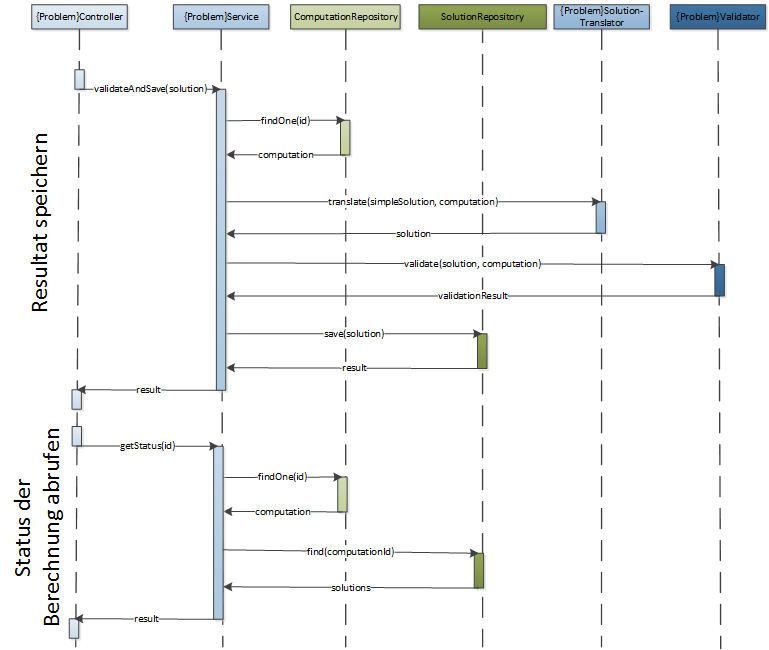
\includegraphics[scale=0.72]{images/visio/sequenz_diagramm_result.png}
\caption[Abspeichern des Resultates eines beliebigen Problemes]{Abspeichern des Resultates eines beliebigen Problemes \selfmade{}}
\label{fig:sequenz_diagramm_result}
\end{figure}

\section{Datenbank Varianten}\label{db_varianten}
Es gibt verschiedene Datenbanktypen und jede hat seine Vor- und Nachteile. In diesem Abschnitt werden vier verschiedenen Typen miteinander verglichen und der beste für diesen 
Anwendungszweck ausgewählt. Um die Eigenheiten der Datenbanken hervorzuheben, wird bei jeder Art das gleiche Beispiel mit der spezifischen Definitions-- und Abfragesprache gemacht.

\subsection{CAP-Theorem}\label{cap_theorem}
Das CAP-Theorem ist im Jahr 2000 aus einer Vermutung von Eric Brewer entstanden \cite{cap_brewer}. Das Theorem zeigt, dass die Werte Konsistenz (C), Verfügbarkeit (A) und Partitionstoleranz (P) ein 
Dreieck (siehe \autoref{fig:cap}) bilden und dass ein verteiltes System nur jeweils zwei dieser Eigenschaften gleichzeitig erfüllen kann.

\begin{figure}[h]
\centering
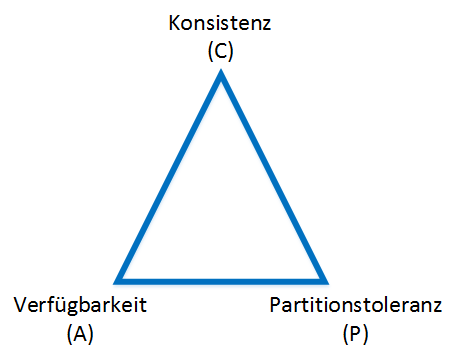
\includegraphics[scale=0.8]{images/visio/cap.png}
\caption[CAP-Theorem]{CAP-Theorem \selfmade{}}
\label{fig:cap}
\end{figure}

\subsubsection{Beispiele}

\begin{itemize}
	\item \textbf{AP}: Domain Name System (DNS), NoSQL Datenbanken
	\item \textbf{CA}: Relationalen Datenbanken
	\item \textbf{CP}: Banken Anwendungen
\end{itemize}

\subsection{Relationales Datenbanksystem}\label{rdbms}
Eine \gls{rdbms} basiert auf Transaktionen und das dazugehörige \gls{acid} Prinzip (vergleiche \cite{limited2010introduction}). 
\begin{itemize}
	\item \textbf{Atomicity}: Eine Reihe von Befehlen wird entweder ganz oder gar nicht ausgeführt.
	\item \textbf{Consistency}: Der Datenzustand ist nach jeder Veränderung wieder konsistent, wenn dies auch vorher der Fall war.
	\item \textbf{Isolation}: Unterschiedliche Befehlsketten beeinflussen sich nicht gegenseitig.
	\item \textbf{Durability}: Vollzogene Änderungen sind dauerhaft, auch bei einem Systemfehler.
\end{itemize}
Beziehungen zwischen Tabellen werden mit Fremdschlüsseln definiert, welche auf den Hauptschlüssel der referenzierten Tabelle zeigt. \autoref{lst:table_definition_rdbms} zeigt die
Tabelle 'Person', welche eine Verbindung zur Tabelle 'Address' hat.

\begin{lstlisting}[language=SQL, caption=Tabellendefinition in relationalem Datenbanksystem, label=lst:table_definition_rdbms]  
    CREATE TABLE ADDRESS(
             ID       INTEGER(11),
             Street   VARCHAR(30),
             Zip      INTEGER(6),
             City     VARCHAR(12));

    CREATE TABLE PERSON(
               ID          INTEGER(11),
               Name        VARCHAR(50),
               FK_Address  INTEGER(11));
\end{lstlisting}

Die Abfrage der Strasse bei einer relationaler Datenbank mittels \gls{sql} ist in \autoref{lst:select_street_rdbms} dargestellt.

\begin{lstlisting}[language=SQL, caption=Abfrage in relationalem Datenbanksystem, label=lst:select_street_rdbms]  
    SELECT ADDRESS.Street
    FROM PERSON 
    JOIN ADDRESS on PERSON.FK_Address = ADDRESS.ID;
    WHERE PERSON.Name = 'Thomas';
\end{lstlisting}

\subsection{Objektrelationales Datenbanksystem}\label{ordbms}
\glslink{ordbms}{Objektrelationale Datenbankmanagementsysteme (ORDBMS)} wurden entwickelt, um das relationale System mit den Funktionen des objektorientierten Stiles zu erweitern.
Die folgende Beschreibung der Eigenschaften ist aus \cite{limited2010introduction} abgeleitet. In objektrelationalen Datenbanksystemen werden 
komplexe Datentypen unterstützt, so können zusätzliche Typen definiert werden und diese können dann bei einer Tabellendefinition verwendet werden.  
In \autoref{lst:type_definition_ordbms} ist eine Typendefinition von 'AddressType' zu sehen, welche wiederum in \autoref{lst:use_type_definition_ordbms} 
in der Tabelle 'Person' verwendet wird.

\begin{lstlisting}[language=SQL, caption=Typendefinition in objektrelationalem Datenbanksystem, label=lst:type_definition_ordbms]  
    CREATE TYPE AddressType  AS
             (Street   VARCHAR(30),
              Zip      INTEGER(6),
              City     VARCHAR(12));
\end{lstlisting}

\begin{lstlisting}[language=SQL, caption=Verwendung von Typendefinition in objektrelationalem Datenbanksystem, label=lst:use_type_definition_ordbms]  
    CREATE TABLE PERSON(
               ID       VARCHAR(20),
               Name     VARCHAR(50),
               Address  AddressType);
\end{lstlisting}

Wenn nun die Strasse einer bestimmten Person abgefragt werden möchte, sieht dies in einer objektrelationaler Datenbank wie in \autoref{lst:select_street_ordbms} aus.

\begin{lstlisting}[language=SQL, caption=Abfrage in objektrelationalem Datenbanksystem, label=lst:select_street_ordbms]  
    SELECT Address.Street
    FROM PERSON;
    WHERE Name = 'Thomas';
\end{lstlisting}

Zusätzlich können auch Arrays von Typen definiert werden, in \autoref{lst:use_array_ordbms} ist die Definition der Tabelle 'Person' mit 
bis zu fünf E-Mail-Adressen gezeigt.

\begin{lstlisting}[language=SQL, caption=Verwendung von Array in objektrelationalem Datenbanksystem, label=lst:use_array_ordbms]  
    CREATE TABLE PERSON(
               ID       VARCHAR(20),
               Name     VARCHAR(50),
               Mail     VARCHAR(40) ARRAY[5]);
\end{lstlisting}

Weiter bieten die Systeme die Möglichkeiten, Methoden auf Typen und Tabellen und Vererbungshierarchien zu definieren. Der Anwendungsbereich 
liegt bei Applikationen, welche viele kurzlebige Transaktionen mit komplexen Objekten durchführen.

\subsection{Objekorientiertes Datenbanksystem}\label{object_db}
Eine \gls{oodbms} hat als Ziel eine bessere und nähere Zusammenarbeit mit objektorientierten Sprachen. 
Die Informationen über \gls{oodbms} sind aus \cite{limited2010introduction} entnommen. Der grosse Unterschied zu anderen Datenbanksystemen
ist die Persistierung, bei \gls{oodbms} wird bereits beim Erstellen eines neuen persistenten Objekts im Code ein Pointer auf das Objekt in der Datenbank zurückgegeben. 
Weiter unterstützen die Systeme Versionierung von Objekten, die Datenbank kann somit mit verschiedenen Versionen der Objekte gleichzeitig umgehen. 
Dies kann bei einer geplanten Umstrukturierung sehr hilfreich sein, wenn die neue Version erst für Tests verwendet wird und die bestehenden Objekte erst nach dem 
Release migriert werden sollen. \autoref{lst:table_definition_oodbms} zeigt, wie das Objekt 'Person' in \gls{odl} definiert wird.

\begin{lstlisting}[language=C++, caption=Objektdefinition in objektorientierem Datenbanksystem, label=lst:table_definition_oodbms]  
    class PERSON
    {
          attribute string Id;
          attribute string Name;
          attribute struct Address
              { string Street,
                short Zip,
                string City} address;
    }
\end{lstlisting}

Für die Abfrage der Strasse einer Person wird ein Statement wie in \autoref{lst:select_street_oodbms} verwendet. Diese Abfragesprache nennt
sich \gls{oql}. Die Attribute der Objekte und Structs können mit einem Punkt separiert verkettet werden.

\begin{lstlisting}[language=SQL, caption=Abfrage in objektorientierem Datenbanksystem, label=lst:select_street_oodbms]  
    SELECT p.Address.Street
    FROM persons p
    WHERE p.Name = 'Thomas';
\end{lstlisting}

Die objektorientierten Datenbanksystemen bietet die aus den \gls{rdbms} bekannten Abfragefunktionen (Avg, Max, Min, Distinct). 
Zusätzlich können bei diesen Systemen Vererbungshierarchien und Methoden in Objekten definiert werden. Sie werden bei Applikationen verwendet,
welche viele und lange Transaktionen mit komplexen Objekten haben.

\subsection{NoSQL Datenbanksystem}\label{no_sql_db}
NoSQL Datenbanksysteme folgen nicht dem \gls{acid} Prinzip, sie sind entwickelt worden, um den erforderlichen Geschwindigkeiten und Grössen von Anwendungen wie Google, 
Facebook, Yahoo und Twitter zu genügen. Die Systeme sind nicht relational aufgebaut und verwenden oft eine andere Abfragesprache als \gls{sql} (siehe \cite{vaish2013getting}). 
Die meisten NoSQL Datenbanksystem setzen auf das \gls{base}-Prinzip von Eric Brewer.

\begin{myQuote}{Gaurav Vaish \cite{vaish2013getting}}
"`\textbf{Basic availability}: Each request is guaranteed a response—successful or failed execution.\\
\textbf{Soft state}: The state of the system may change over time, at times without any input (for eventual consistency).\\
\textbf{Eventual consistency}: The database may be momentarily inconsistent but will be consistent eventually."'
\end{myQuote}

Nahe zu alle NoSQL Datenbanksysteme sind schemalos, dass heisst, die Tabellen müsse nicht im Vorherein definiert werden. Die Abfragen gestalten sich einfach, JOIN Befehle entfallen 
komplett. Durch den lockeren Aufbau kann eine höhere Performance erzielt werden, die Unterschiede bei der Geschwindigkeit werden bereits bei kleineren Datenmengen bemerkbar.

\subsubsection{NoSQL Datenbanktypen}\label{no_sql_db_subgroups}
NoSQL ist eine Übergruppe von unterschiedlichen Datenbanktypen. In diesem Abschnitt wird auf drei verschiedene NoSQL Datenbanktypen eingegangen, die Eigenschaften der jeweiligen
 Typen sind aus \cite{vaish2013getting} entnommen.

\paragraph{Document}
Bei dokumentorientierten Datenbanken werden \gls{semi_structured_data} abgespeichert, diese verwenden meistens die Dateiformate \gls{json}, 
\gls{xml} oder \gls{yaml}. Die meisten Datenbanksysteme dieser Art haben kein definiertes Schema für Einträge oder 
nur ein teilweise definiertes Schema. Es ist somit möglich ganz unterschiedliche Elemente in eine Tabelle bzw. Collection, so werden Tabellen in dieser Welt genannt, zu speichern. Diese Erklärung 
erinnert an \gls{blob} in relationalen Datenbanken, jedoch können hier Indexes auf bestimmte Attribute gesetzt und innerhalb der Elemente effizient gesucht 
werden.

In \autoref{lst:person_mongodb} wird ein Personen Element gezeigt, welches in der Collection 'Persons' gespeichert ist. Dieses Beispiel ist basierend auf einer MongoDB Instanz, die Definition 
für die Collection entfällt komplett.

\begin{lstlisting}[language=JSON, caption=Personen Element in JSON Format, label=lst:person_mongodb]  
    {
       _id: 1,
       name: "Thomas",
       address: {
                 street: "Bahnhofstrasse 45",
                 zip: 8315,
                 city: "Lindau"}
    }
\end{lstlisting}

\autoref{lst:select_mongodb} zeigt die Abfrage der Strasse bei MongoDB, welche das Resultat aus \autoref{lst:select_result_mongodb} liefert. Bei MongoDB wird bei einer Abfrage standardmässig 
immer das ganze Element zurückgegeben, falls nur gewiese Attribute abgefragt werden sollen, können diese in dem Projektionsabschnitt definiert werden. Die ID des Elements wird, so lang 
sie nicht explizit ausgeschlossen wird, immer mit selektiert.

\begin{lstlisting}[language=SQL, caption=Abfrage in MongoDB, label=lst:select_mongodb]  
    db.persons.find({name: "Thomas"}, {_id: 0, "address.street": 1})
\end{lstlisting}

\begin{lstlisting}[language=JSON, caption=Resultat der Abfrage in MongoDB, label=lst:select_result_mongodb]  
    {
       address: {
                 street: "Bahnhofstrasse 45"}
    }
\end{lstlisting}

\paragraph{Column-oriented}
Anders als bei relationalen Datenbanken, welche zeilenorientierte sind, werden die Daten spaltenorientiert gespeichert. Eine Lohndatenbank würde serialisiert beim zeilenorientierten Konzept
wie in \autoref{lst:ser_rowbased_db} und beim spaltenorientierten Ansatz wie in \autoref{lst:ser_columnbased_db} aussehen.

\begin{lstlisting}[language=SQL, caption=Serialisierung zeilenorientierte Datenbank, label=lst:ser_rowbased_db]  
    1,Thomas,100000
    2,Patrick,120000
    3,Andreas,200000
\end{lstlisting}

\begin{lstlisting}[language=SQL, caption=Serialisierung spaltenorientierte Datenbank, label=lst:ser_columnbased_db]  
    1,2,3
    Thomas,Patrick,Andreas
    100000,120000,200000
\end{lstlisting}

Die Definitions- und Abfragesprache ist gleich wie bei relationalen Datenbanken, deshalb wird hier auf Beispiele verzichtet. Der Vorteil 
einer spaltenorientierten Datenbank liegt in der Performance bei \glspl{aggregationsfunktion}. Weiter führt dieser Datenbanktyp Veränderungen, 
welche alle Werte einer Spalte betreffen, effizient durch. Dafür ist das Einfügen einer neu Zeile oder das Auslesen einer ganze Zeile aufwendiger als bei dem zeilenorientierten Ansatz.

\paragraph{Graph}
In Graphdatenbanken sind die abgespeicherten Objekte die Knoten und die Beziehung der Objekte bilden die Kanten. Die Kanten können zusätzlich mit Eigenschaften versehen werden. Dieser 
Datenbanktyp kann für komplexe Netzwerke verwendet werden. Der Vorteil liegt bei der Handhabung der Beziehungen. Das Herausfinden der kürzesten Route zwischen zwei Elementen über 
ihre definierten Beziehungen stellt für diesen Datenbanktyp keine Herausforderung dar.

Die Daten werden je nach Implementation auch in Dokumenten abgespeichert, somit entfällt auch hier eine Definition des Schemas. In \autoref{lst:select_neo4j} ist das Beispiel 
für das Abfragen der Strasse einer Person in Neo4j zu sehen.

\begin{lstlisting}[language=SQL, caption=Abfrage in Neo4j, label=lst:select_neo4j]  
       MATCH (person:Person)
       WHERE person.name = "Thomas"
       RETURN person.address.street;
\end{lstlisting}

\subsection{Vorselektierung}\label{preselection}
Um nicht alle sechs vorgestellten Datenbanksysteme in der Nutzwertanalyse miteinander vergleichen zu müssen, wurde eine Vorselektierung aufgrund der Ist-Analyse gemacht. Da 
objektrelationale und objektorientierte Datenbanksystem eher akademischer Natur sind und keine detaillierte Dokumentation darüber gefunden wurde, werden sie von der Nutzwertanalyse 
ausgeschlossen. Die Anforderungen lassen auf keinen Anwendungsfall für eine spaltenorientierte Datenbank schliessen. In den einzelnen Problemen spielen Beziehungen zwischen Objekten 
zwar oft eine Rolle, doch das würde eher in den Bereich des Algorithmus fallen, aus diesem Grund werden Graphdatenbanken ebenfalls ausgeschlossen. Somit bleiben noch die relationale 
Datenbank und die dokumentorientierten Datenbanken für die Nutzwertanalyse übrig.

Da es innerhalb der ausgewählten Datenbanksystemen sehr viele verschiedene Implementationen gibt, wurde von jedem Typ eine ausgewählt. Bei den relationalen Datenbanken fiel die 
Entscheidung auf MySQL, da diese Implementation kostenlos ist und bereits Erfahrung vorhanden war. Da MongoDB sehr verbreitet und eine gute Integration in die Java Frameworks hat, 
wurde diese Implementation unter den dokumentorientierten Datenbanken ausgewählt.

\newpage
\section{Nutzwertanalyse}\label{architektur_nutzwertanalyse}

\subsection{Bewertungskriterien}\label{architektur_bewertungspunkte}

In der Nutzwertanalyse werden folgende Punkte betrachtet und nach dem angegebenen Schema bewertet und dann gewichtet. 
Die Kriterien sind grösstenteils aus den \gls{cap_theorem} abgeleitet.

\paragraph{Aufwand}
\begin{itemize}
	\item \textbf{Beschreibung}: Wie gross ist der geschätzte Aufwand mit diesem Datenbanktyp?
	\item \textbf{Bewertung}: 1: sehr hoch, 10: sehr niedrig
	\item \textbf{Gewichtung}: 5 (Die Zeit für dieses Projekt ist beschränkt und die Entscheidung könnte zu einem Risiko werden.)
\end{itemize}

\paragraph{Änderbarkeit}
\begin{itemize}
	\item \textbf{Beschreibung}: Wie flexibel ist diese Variante in Bezug auf Erweiterungen/Vererbung?
	\item \textbf{Bewertung}: 1: sehr spezifisch, 10: sehr flexibel
	\item \textbf{Gewichtung}: 5 (Die Anforderungen geben vor, dass das System einfach zu erweitern sein sollte.)
\end{itemize}

\paragraph{Konsistenz}
\begin{itemize}
	\item \textbf{Beschreibung}: Wie gut ist die Datenbank in Bezug auf Konsistenz?
	\item \textbf{Bewertung}: 1: gar nicht 10: sehr gut
	\item \textbf{Gewichtung}: 2 (Die Daten haben untereinander so gut wie keine Abhängigkeiten, es werden fast nur Einfüge-Operationen benützt.)
\end{itemize}

\paragraph{Verfügbarkeit}
\begin{itemize}
	\item \textbf{Beschreibung}: Wie hoch ist die Verfügbarkeit der Datenbank-Operationen?
	\item \textbf{Bewertung}: 1: niedrig, 10: sehr hoch
	\item \textbf{Gewichtung}: 4 (Die Schnittstelle wird für möglichst viele gleichzeitige Requests ausgelegt, eine Warteschlaufe von Operationen ist nicht gewünscht.)
\end{itemize}

\paragraph{Partitionstoleranz}
\begin{itemize}
	\item \textbf{Beschreibung}: Kann die Datenbank verteilt betrieben werden?
	\item \textbf{Bewertung}: 1: nur eingeschränkt, 10: sehr einfach
	\item \textbf{Gewichtung}: 4 (Mit zunehmender Grösse wird die Datenbank sehr wahrscheinlich verteilt betrieben.)
\end{itemize}

\newpage
\subsection{Bewertung}\label{architektur_bewertung}
Anhand der zuvor definierten Kriterien wurde eine Bewertung vorgenommen. Diese Bewertung ist nicht generell gültig, sie bezieht sich nur auf dieses Projekt.

\begin{table}[ht]
\centering
  \begin{tabular}{>{\columncolor{darkgray}} l | p{5cm} | p{5cm}}
	\hline
	\rowcolor{darkgray}
	\textbf{Kriterium}		&	\textbf{Relationale Datenbank} 	&	\textbf{Dokumentorientierte Datenbank}	\\ \hline
	\rowcolor{gray}
	Aufwand		&	7 (35)		&	7 (35)		\\ \hline
	Begründung		&	MySQL ist bekannt und das Einrichten ist relativ schnell gemacht.			
				&	Dokumentorientierten Datenbank noch nie benutzt. Laut Informanten ziemlich simpel.	\\ \hline
	\rowcolor{gray}
	Änderbarkeit		&	3 (15)		&	10 (50)		\\ \hline
	Begründung		&	Jede Anpassung an den Entities Attributen erfordert auch eine Änderung des Schemas.
				&	Sehr flexibel, bei Änderungen der Entities oder neuen Probleme keine Anpassung nötig.\\ \hline
	\rowcolor{gray}
	Konsistenz		&	10 (20)	&	4 (8)		\\ \hline
	Begründung		&	Konsistenz ist einer der Hauptgründe für relationale Datenbanksysteme.			
				&	Die Stärke liegt nicht in der Konsistenz.\\ \hline
	\rowcolor{gray}
	Verfügbarkeit	&	6 (24)	&	9 (36)		\\ \hline
	Begründung		&	Bei Transaktionen sind oft Teile der Datenbank gesperrt und nicht verfügbar.					
				&	Keine Sperrzeiten von Einträgen, somit keine Verzögerungen von Aktionen.	\\ \hline
	\rowcolor{gray}
	Partitionstoleranz	&	7 (28)	&	9 (36)		\\ \hline
	Begründung		&	Benötigt aufwendige Konfiguration um die Datenbank verteilt zu betreiben.
				&	Kann gut und einfach verteilt betrieben werden.		\\ \hline \hline
	\rowcolor{gray}
	\textbf{Total (gewichtet)}	&	\textbf{33 (122)}	&	\textbf{39 (165)}	\\ \hline
  \end{tabular}
   \caption{Nutzwertanalyse - Datenbank Varianten}\label{table:bewertungskriterien}
\end{table}

\FloatBarrier
\subsection{Fazit}\label{architektur_fazit}
Das Resultat der Nutzwertanalyse hat ergeben, dass für dieses Projekt am besten eine dokumentorientierte Datenbank Lösung verwendet wird.
Die Schnittstelle benötigt keine Transaktionen und profitiert von einer hohen Verfügbarkeit und Partitionstoleranz. Die Flexibilität
von dokumentorientierten Datenbanksystemen ist ideal für dieses Projekt, da sie eine schnelle und unkomplizierte Erweiterung bzw. Anpassung ermöglicht. Zusätzlich werden 
auch die verschiedenen Ausprägungen der einzelnen Problemen gut unterstützt.

\section{Datendiagramm des Datenspeichers}\label{datendiagramm_datenspeicher}
Da sich bei der Nutzerwertanalyse ergeben hat, dass eine dokumentorientierte Datenbank verwendet wird, entfällt ein Datendiagramm der Tabellen, wie es von relationalen Datenbanken 
bekannt ist. Die Collections benutzen kein vordefiniertes Schema, jedoch legen die verwendeten Klassen, welche in die Collections gespeichert werden, das Schema fest. Aus diesem Grund 
reicht ein Klassendiagramm, um zu wissen, wie die Daten abgespeichert werden.

In \autoref{fig:problems_diagramm} ist die Klassen-Hierarchie der Berechnungstypen dargestellt und in \autoref{fig:solutions_diagramm} werden die verschiedenen 
Resultatklassen gezeigt.


\begin{figure}[h]
\centering
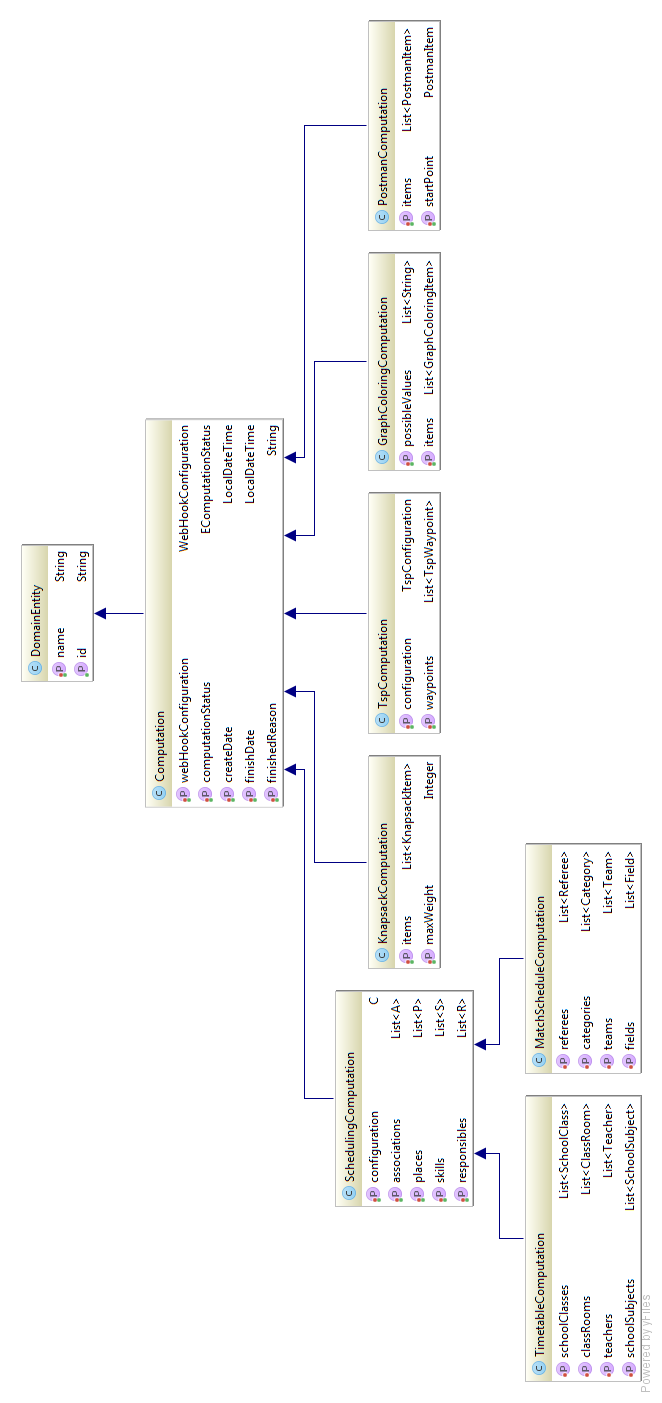
\includegraphics[scale=0.62]{images/computations_diagramm.png}
\caption[Klassendiagramm der verschiedenen Problemklassen]{Klassendiagramm der verschiedenen Problemklassen \selfmade{}}
\label{fig:problems_diagramm}
\end{figure}

\begin{figure}[h]
\centering
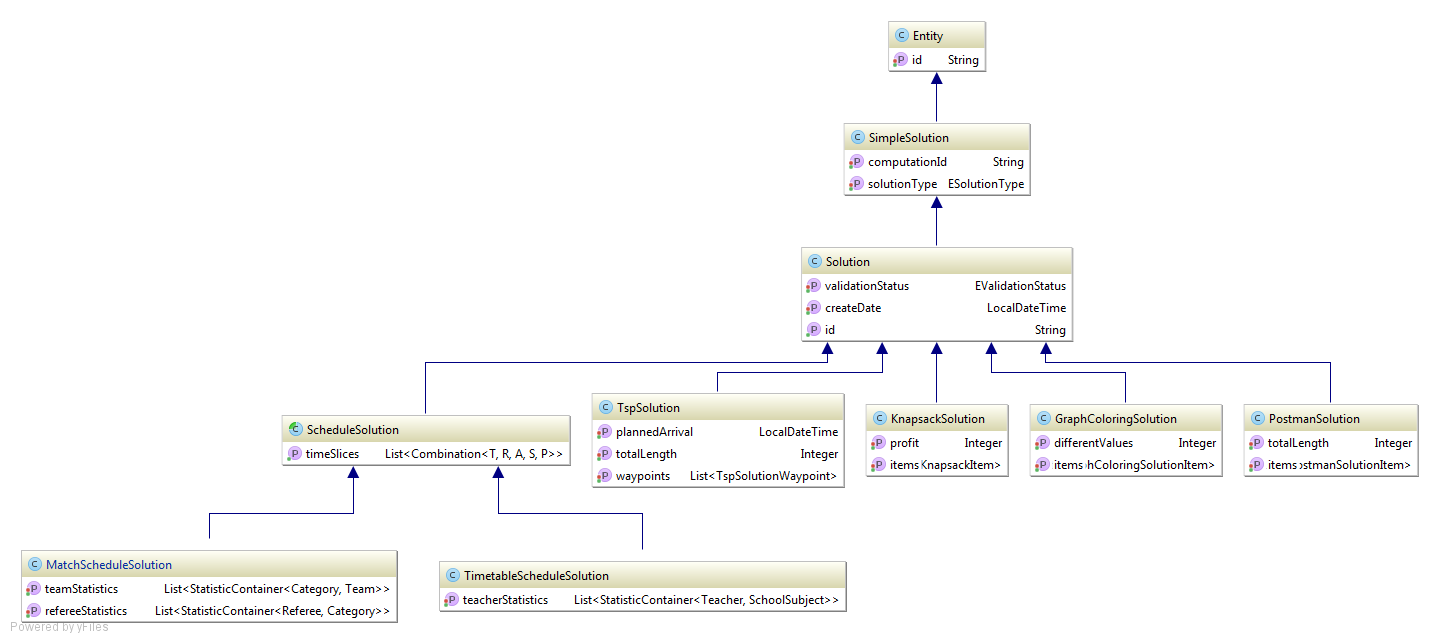
\includegraphics[scale=0.6]{images/solutions_diagramm.png}
\caption[Klassendiagramm der verschiedenen Resultatklassen]{Klassendiagramm der verschiedenen Resultatklassen \selfmade{}}
\label{fig:solutions_diagramm}
\end{figure}
